\documentclass{article}
\usepackage{graphicx}
\usepackage{geometry}
\usepackage{tabularx}
\usepackage{float} % Paquete necesario para usar [H] y forzar posiciones
\usepackage{caption} % Para mejor control de los títulos

% Configuración de geometría
\geometry{
  letterpaper,
  top=2cm,
  bottom=2.5cm,
  left=2cm,
  right=2cm
}

\setlength{\columnsep}{1cm}
\twocolumn

\title{Práctica Experimental \\ Emparejamiento Estable}
\author{Gonzalez Lugo Arlet Linette}
\date{Febrero 2026}
\raggedbottom

\begin{document}
\maketitle

\begin{abstract}
\textbf{Este documento presenta el desarrollo experimental del algoritmo de emparejamiento estable propuesto por Gale y Shapley y su análisis de comportamiento mediante la generación de múltiples instancias del problema Stable Matching Problem (SMP) y la medición de tiempos de ejecución.}
\end{abstract}

\renewcommand{\thesection}{\Roman{section}}

\section{Introducción}
Se desarrollará una práctica experimental que implica la implementación y ejecución del algoritmo de emparejamiento estable propuesto por Gale y Shapley, el cual proporciona una solución formal al problema conocido como Stable Matching Problem (SMP). Asimismo, se realizará un análisis de su comportamiento y rendimiento bajo diversos conjuntos de datos y escenarios de prueba.

\section{Objetivo}
El objetivo de esta práctica es comprobar experimentalmente el comportamiento del algoritmo de Gale y Shapley, que encuentra el emparejamiento estable entre dos conjuntos de hombres y mujeres cuya cardinalidad es $N$. Es decir, resolver el SMP y analizar su tiempo de ejecución conforme aumenta el tamaño del problema.

\section{Metodología Experimental}
Esta sección describe el procedimiento experimental llevado a cabo para cumplir con el objetivo. Se utilizó el IDE Visual Studio Code como entorno de desarrollo.

\subsection{Implementación del algoritmo en Python}
El programa fue dividido en dos funciones principales: \texttt{main} y \texttt{gale\_shapley}. En la función \texttt{gale\_shapley} se implementa el algoritmo de emparejamiento estable.

La Figura~\ref{fig:gale} muestra el diagrama de flujo del algoritmo implementado.

\begin{figure}[H] % [H] fuerza la posición exacta
\centering
\includegraphics[width=0.9\linewidth]{diagrama.png}
\caption{Diagrama de flujo del algoritmo Gale-Shapley}
\label{fig:gale}
\end{figure}

\subsection{Generación automática de archivos de prueba}
Se implementó un generador de instancias utilizando las librerías \texttt{random} y \texttt{os}. La metodología consiste en generar archivos de texto, cada uno correspondiente a un tamaño específico del problema que aumenta en múltiplos de 8 y 80.

Para cada archivo:
\begin{itemize}
    \item Se generan identificadores desde H1 hasta Hn.
    \item Se generan identificadores desde M1 hasta Mn.
    \item Se crea una permutación aleatoria completa de mujeres y hombres mediante \texttt{random.shuffle}.
\end{itemize}

De esta manera se garantiza que cada individuo tenga una lista de preferencias completa y única.

\subsection{Ejecución del algoritmo}
El programa del algoritmo de Gale y Shapley se ejecutó para cada archivo generado, procesando automáticamente todas las instancias creadas.

\subsection{Medición de tiempos}
Se registraron los tiempos de ejecución correspondientes a cada tamaño de entrada con el objetivo de analizar experimentalmente el comportamiento asintótico del algoritmo, empleando para ello el lenguaje de programación Python.  

La medición de tiempos se efectuó mediante la función \texttt{time.perf\_counter()}, la cual proporciona la mayor resolución disponible para la estimación de intervalos de tiempo cortos. Cada tiempo de ejecución se expresó en milisegundos, obteniéndose dicho valor a partir del producto del tiempo medido por 1000.  

Los resultados fueron almacenados en un archivo de texto \texttt{(resultados\_gale\_shapley.txt)}, que contiene el nombre del archivo de entrada, el número de parejas y el tiempo de ejecución asociado, junto con estadísticas como los valores mínimo, máximo y promedio.

\subsection{Tiempos de ejecución}
A continuación se presentarán dos tablas. La primera corresponde a la Tabla 1, construida a partir de 80 archivos, cuyos valores incrementan en múltiplos de 8. La segunda tabla se obtuvo a partir de 100 archivos, con valores que incrementan en múltiplos de 80.

\begin{table}[H] % [H] fuerza la posición exacta
  \centering
  \caption{Tiempos de ejecución para 80 archivos con incrementos de 8}
  \label{tab:tabla1}
  \begin{tabularx}{0.48\textwidth}{|X|c|r|}
    \hline
    Archivo & N & Tiempo (ms) \\
    \hline
    1  & 8   & 0.0148  \\
    \hline
    2  & 160 & 0.5640  \\
    \hline
    3  & 320 & 3.0848  \\
    \hline
    4  & 480 & 11.8335 \\
    \hline
    5  & 640 & 19.3792 \\
    \hline
  \end{tabularx}
\end{table}

En la primera tabla se usan 5 archivos con 8, 160, 320, 480 y 640 parejas. Los tiempos van de 0.0148 a 19.3792 milisegundos y se observa un incremento a partir del archivo 3, con 320 parejas.

\begin{table}[H] % [H] fuerza la posición exacta
  \centering
  \caption{Tiempos de ejecución para 100 archivos con incrementos de 80}
  \label{tab:tabla2}
  \begin{tabularx}{0.48\textwidth}{|X|c|r|}
    \hline
    Archivo & N & Tiempo (ms) \\
    \hline
    1  & 80   & 0.1911    \\
    \hline
    2  & 1600 & 118.5043  \\
    \hline
    3  & 3200 & 439.2357  \\
    \hline
    4  & 4800 & 961.8948  \\
    \hline
    5  & 6400 & 2374.9481 \\
    \hline
    6  & 8000 & 2668.5654 \\
    \hline
  \end{tabularx}
\end{table}

En la segunda tabla se usan 6 archivos con 80, 1600, 3200, 4800, 6400 y 8000 parejas.

\subsection{Realización de Gráficas y su análisis}
La implementación gráfica se realizó utilizando Python con la biblioteca \texttt{matplotlib}. Cada cinco archivos se realizaba un muestreo, a partir del cual se obtenían los valores (n, tiempo) para su posterior visualización.

Las gráficas incluyen un recuadro con estadísticas resumidas en la esquina superior izquierda, que muestra el número de archivos procesados, así como los tiempos mínimo, máximo y promedio.

\section{Resultados}
En esta sección se presentarán las gráficas y el análisis comparativo del crecimiento temporal observado respecto al tamaño $N$.

\subsection{Resultados para incrementos de 8}
\begin{figure}[H]
\centering
\includegraphics[width=0.9\linewidth]{tiempos.png}
\caption{Gráfica lineal para 80 archivos con múltiplos de 8}
\label{fig:lineal8}
\end{figure}

En la Figura~\ref{fig:lineal8} se observa un crecimiento aproximadamente lineal en el tiempo de ejecución a medida que aumenta el número de parejas. Los puntos se distribuyen alrededor de una línea recta con cierta dispersión. Existe una variabilidad notable en los tiempos, especialmente para valores grandes de n, donde los puntos muestran una banda de dispersión más amplia.

\begin{figure}[H]
\centering
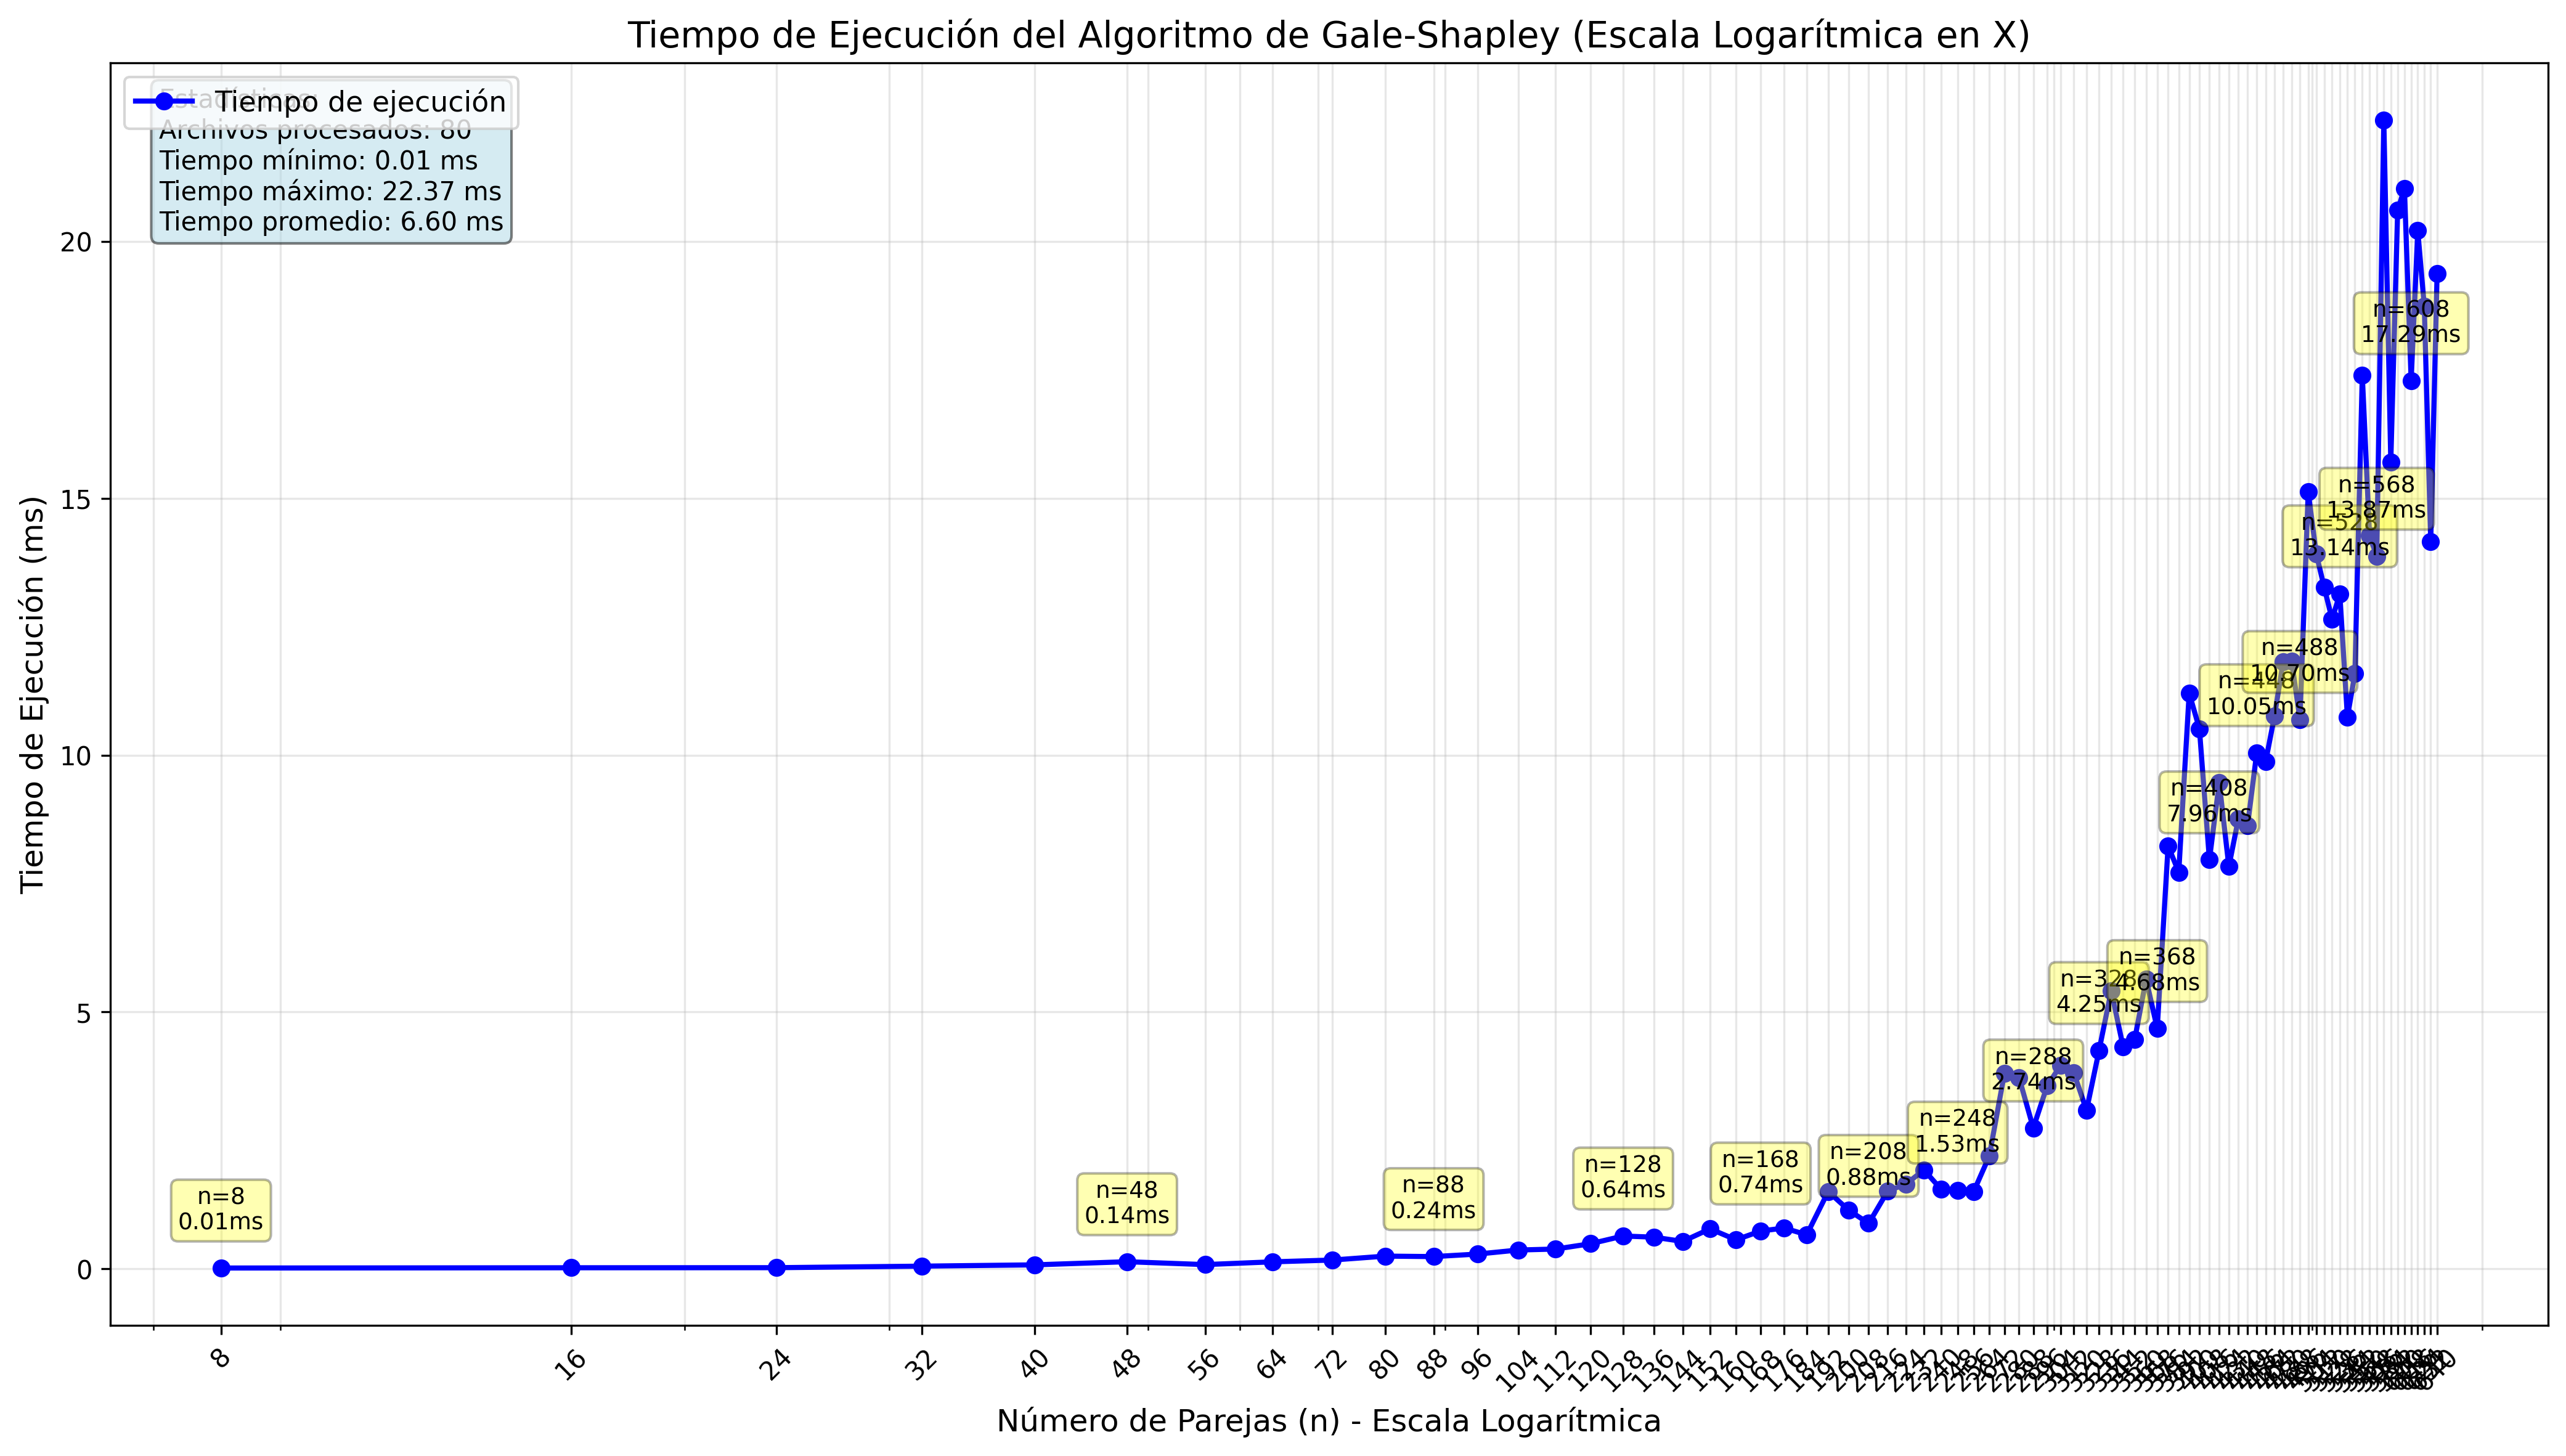
\includegraphics[width=0.9\linewidth]{tiempos_log2.png}
\caption{Gráfica semilogarítmica (eje x log) para 80 archivos con múltiplos de 8}
\label{fig:log8}
\end{figure}

La gráfica con escala logarítmica en el eje X (Figura~\ref{fig:log8}) revela que el algoritmo de Gale-Shapley mantiene un comportamiento consistente y predecible en todo el rango analizado desde 8 hasta 640 parejas. Los puntos se distribuyen uniformemente mostrando una tendencia aproximadamente lineal, lo que sugiere una relación de tipo potencial donde el tiempo de ejecución crece de forma controlada. Los tiempos registrados van desde 0.01 ms para las instancias más pequeñas hasta 22.37 ms para las más grandes, con un promedio de 6.60 ms, lo que confirma la eficiencia práctica del algoritmo para los tamaños de problema evaluados.

\subsection{Resultados para incrementos de 80}
\begin{figure}[H]
\centering
\includegraphics[width=0.9\linewidth]{tiempos2.png}
\caption{Gráfica lineal para 100 archivos con múltiplos de 80}
\label{fig:lineal80}
\end{figure}

\begin{figure}[H]
\centering
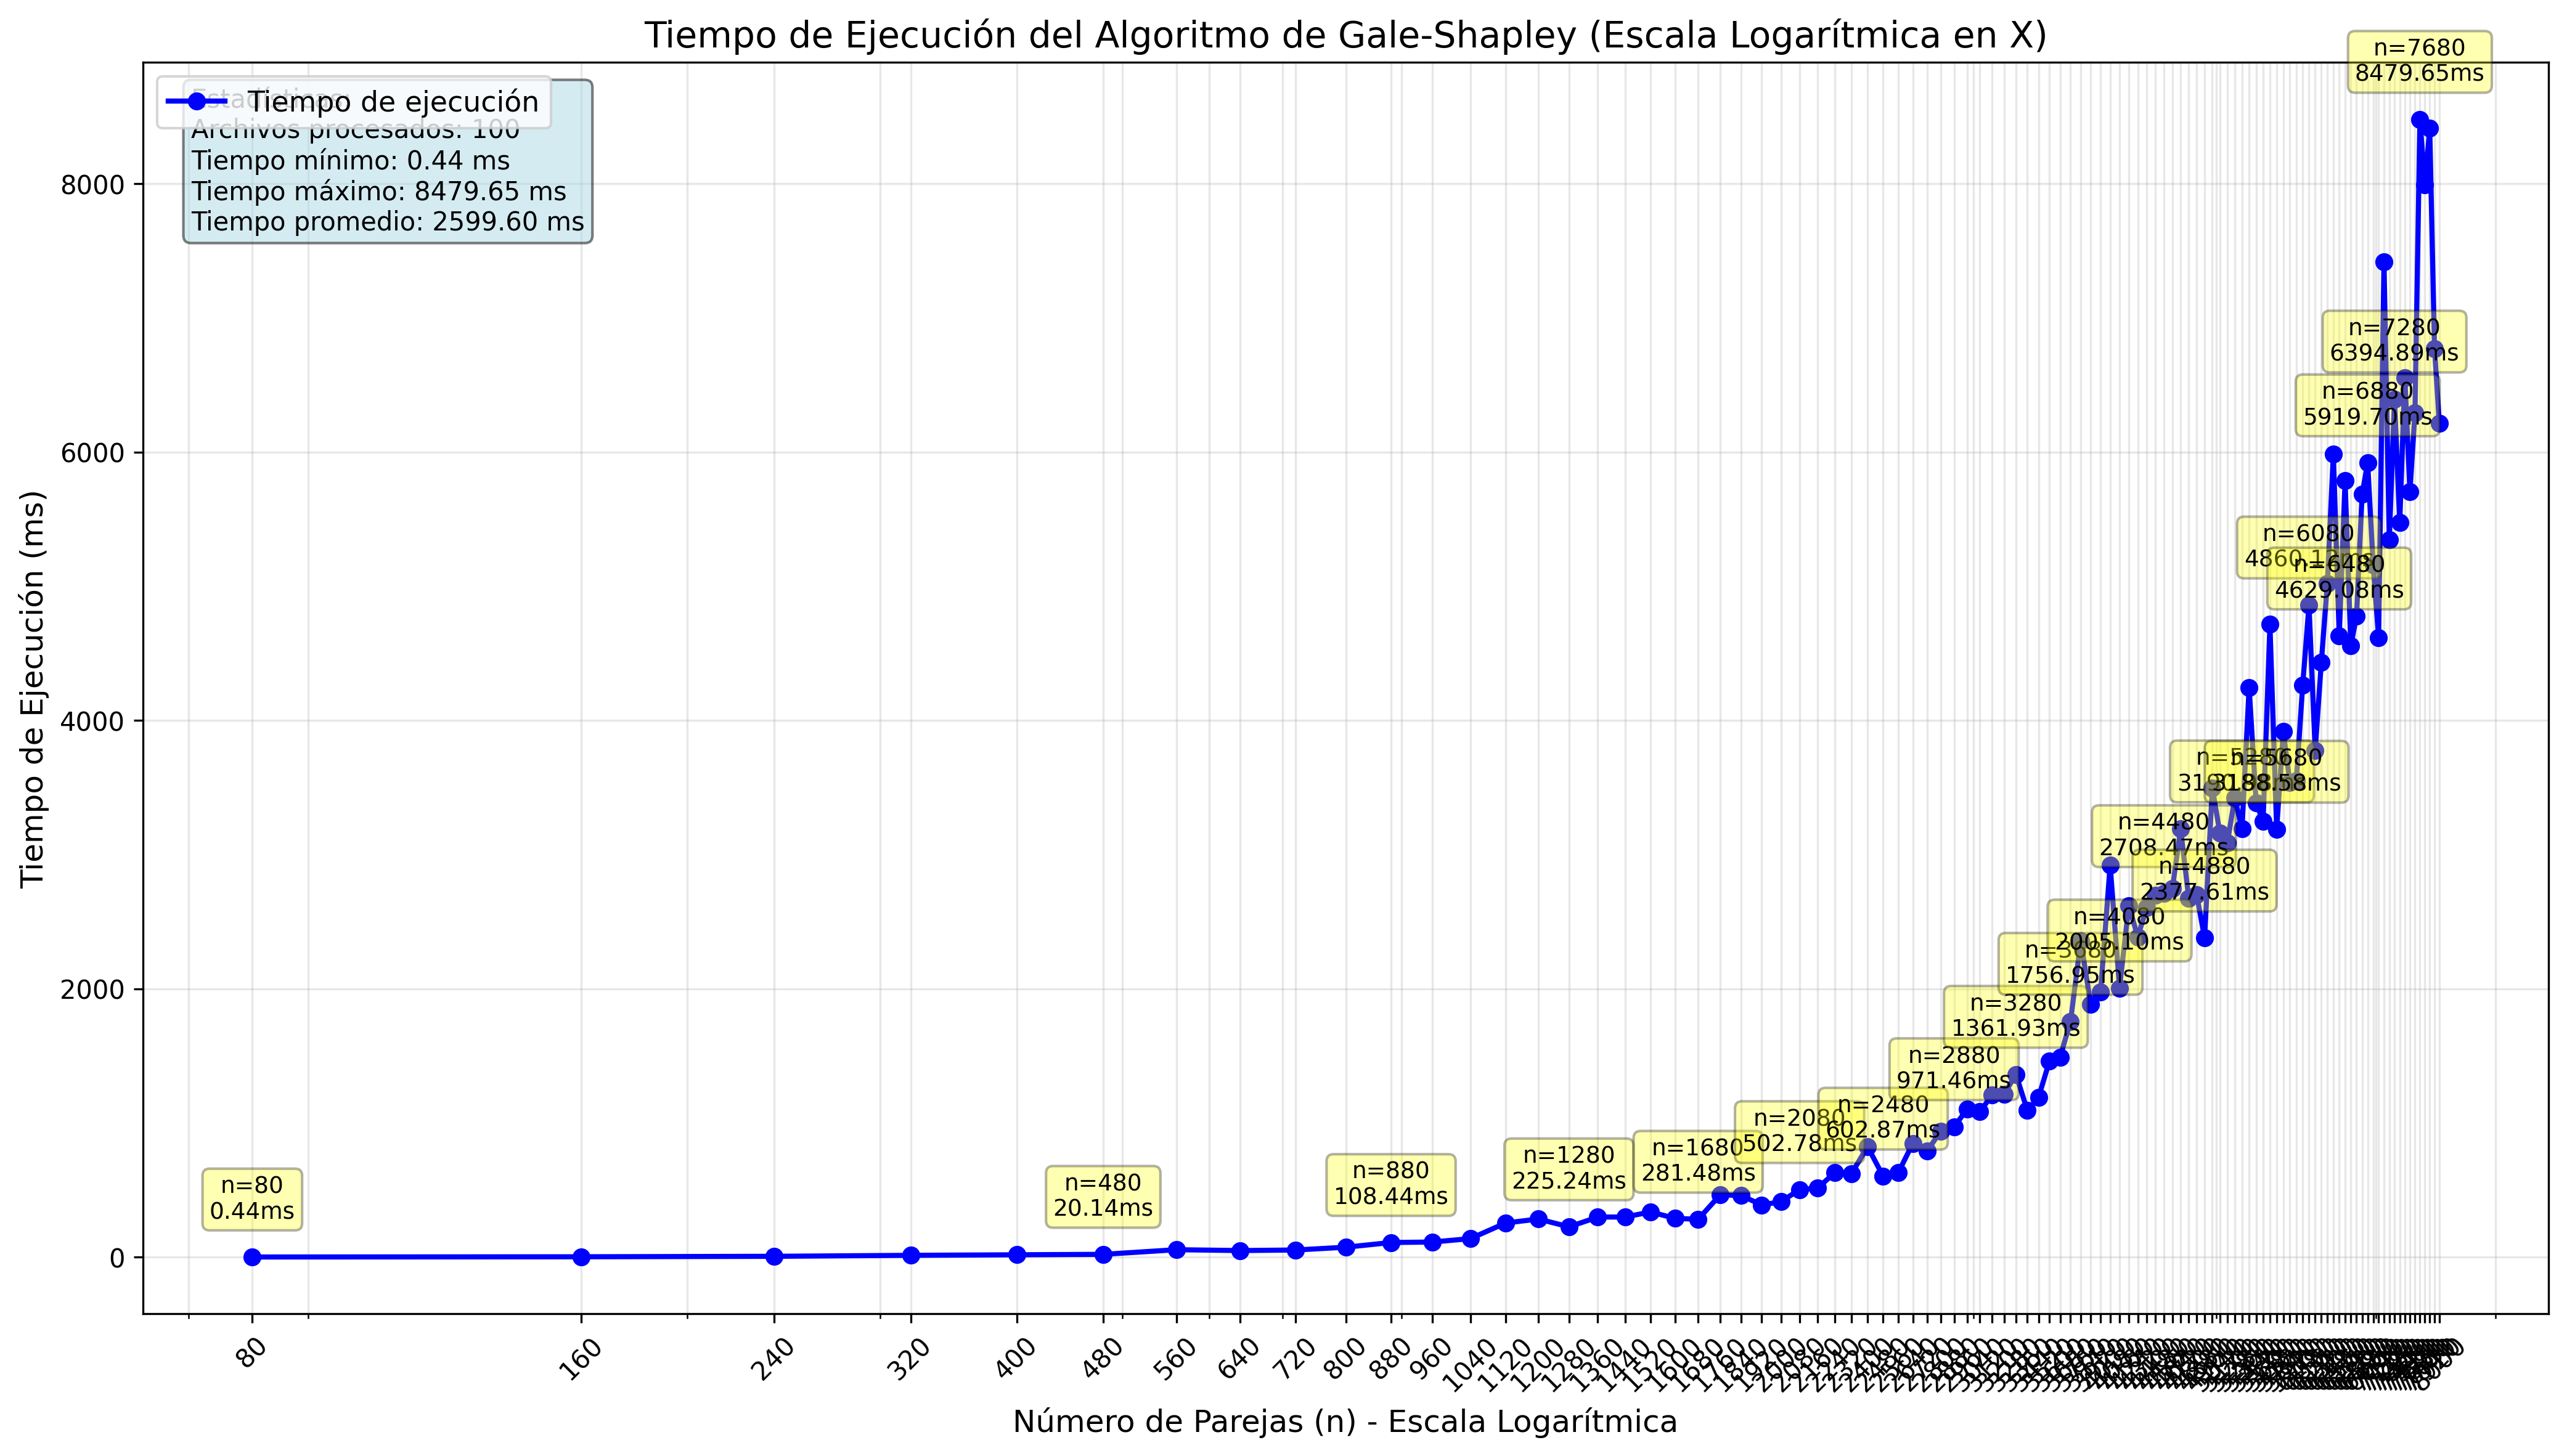
\includegraphics[width=0.9\linewidth]{tiempos_log22.png}
\caption{Gráfica semilogarítmica (eje x log) para 100 archivos con múltiplos de 80}
\label{fig:log80}
\end{figure}

\section{Conclusiones}
Como podemos observar en las Figuras~\ref{fig:log8} y~\ref{fig:log80} con escala logarítmica en el eje X, se revela de forma contundente el comportamiento asintótico del algoritmo de Gale-Shapley. Particularmente en la Figura~\ref{fig:log80}, para instancias de gran tamaño, se observa un crecimiento más que lineal en el tiempo de ejecución a medida que aumenta el número de parejas, evidenciado por el incremento drástico desde 0.44 ms para las instancias más pequeñas hasta 8479.65 ms para las de mayor tamaño.

Esta tendencia ascendente y no lineal es consistente con la complejidad teórica del algoritmo, que es $O(n^2)$ en el peor caso. La escala logarítmica en el eje de las abscisas permite apreciar que, aunque el crecimiento no es exponencial, el tiempo de ejecución se incrementa de manera significativa y sostenida, lo que evidencia la dependencia cuadrática del algoritmo respecto al tamaño de la entrada. Este comportamiento valida experimentalmente las predicciones teóricas y demuestra que, para instancias de gran escala, el costo computacional puede volverse considerable, lo cual es fundamental considerar en aplicaciones prácticas que requieran emparejamientos estables con un número elevado de participantes.

\end{document}